\documentclass[12pt,a4paper]{report}

\usepackage[utf8]{inputenc}
\usepackage{amsmath}
\usepackage{amsfonts}
\usepackage{amssymb}
\usepackage{hyperref}
\usepackage{graphicx}
\usepackage{titlesec}
\usepackage{booktabs}
\usepackage{eurosym}
\usepackage[table]{xcolor}
\usepackage[francais]{babel}
\usepackage[left=2cm,right=2cm,top=2cm,bottom=2cm]{geometry}

\newcommand{\CMName}{\#currentmood}

% Personnalisation des chapitres
\titleformat{\chapter}[hang]
{\fontfamily{cmss}\bfseries\huge}{\Roman{chapter} -- }{0cm}{%
	\vspace{1ex}
}

% Personnalisation des sections
\titleformat{\section}[hang]
{\bfseries\Large}{\arabic{section} -- }{0cm}{%
	\vspace{1ex}
}

% Personnalisation des tableaux
\arrayrulecolor{lightgray}

\title{PJE\\\CMName}
\author{Quentin Van de Kadsye \and Jérôme Tanghe}
\date{Mardi 15 décembre 2015}

\setlength{\parskip}{\baselineskip}

\begin{document}
\maketitle

\tableofcontents

% -----------------------------------------------------------------------------

\chapter{Le projet}

Il est parfois intéressant pour les entreprises de connaître l'humeur générale
des gens concernant un sujet donné. Twitter étant une plateforme où l'on peut
s'exprimer librement, c'est donc un emplacement de choix pour récolter ce type
d'information. Se pose alors le problème suivant : comment connaître rapidement
l'humeur des personnes sur un sujet donné?

Nommé selon le hashtag du même nom, \textbf{\CMName} est un programme tentant de
répondre à ce besoin. Écrit en Java, il permet d'estimer l'humeur d'un ou
plusieurs messages publiés sur Twitter (\textit{tweet}), à l'aide d'une des trois méthodes proposées:

\begin{itemize}
	\item
		\textbf{Mots-clés:} utilise une liste de mots prédéfinis dans des
		fichiers pour déterminer l'humeur du tweet.
	\item
		\textbf{KNN:} évalue l'humeur d'un tweet en fonction de l'humeur de $k$
		autres tweets, en recherchant dans une base de données de tweets dont on
		connaît déjà l'humeur ceux qui contiennent les mêmes mots.
	\item
		\textbf{Classification bayésienne:} évalue la probabilité d'humeur d'un
		tweet en calculant la probabilité que les mots qu'il contient
		appartiennent à cette humeur à partir de la base de données.
\end{itemize}

Le code source du logiciel est disponible sur GitHub:
\href{http://github.com/Deuchnord/currentmood}{github.com/Deuchnord/currentmood}.

\begin{figure}
	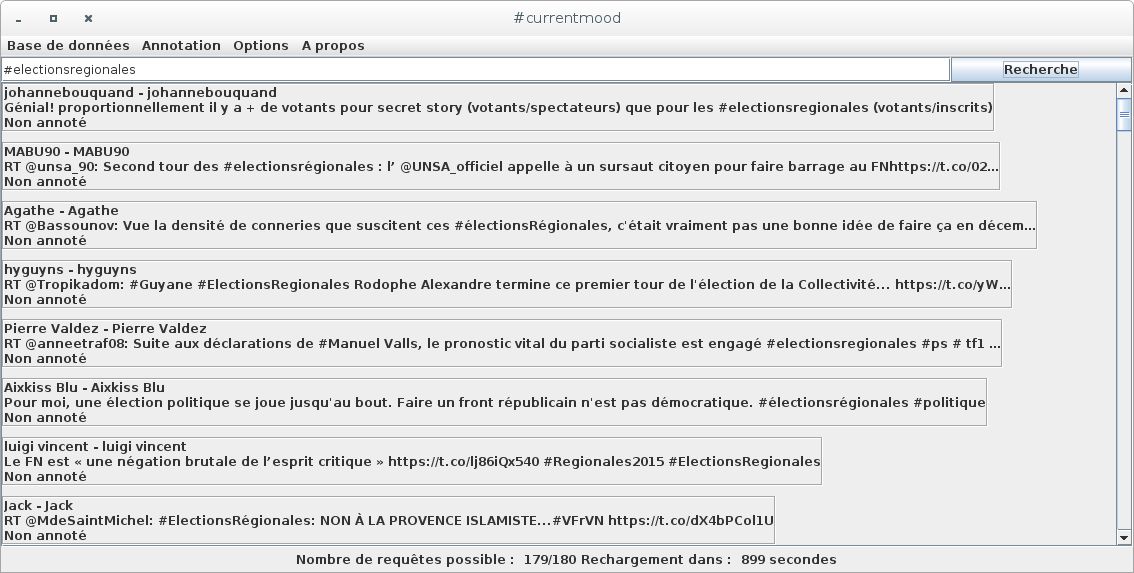
\includegraphics[width=\textwidth]{img/capture-currentmood-ui.png}
	\caption{Interface utilisateur générale de \CMName}
	\label{cm_ui}
\end{figure}


% -----------------------------------------------------------------------------
\chapter{L'interface de \CMName}


% -----------------------------------------------------------------------------

\chapter{API Twitter et gestion des tweets}

\section{La classe \texttt{CMTwitter}}

Afin de communiquer avec l'API de Twitter, nous avons utilisé la librairie
\textbf{Twitter4J}\footnote{\href{http://twitter4j.org}{twitter4j.org}} qui
propose les fonctionnalités dont nous avons besoin pour mener à bien le projet.
Pour faciliter son implémentation, nous avons également créé une classe,
\texttt{CMTwitter}, s'interfaçant entre notre application et Twitter4J, comme le
montre la figure~\ref{uml_cmtwitter} (page~\pageref{uml_cmtwitter}).

\begin{figure}%[h]
	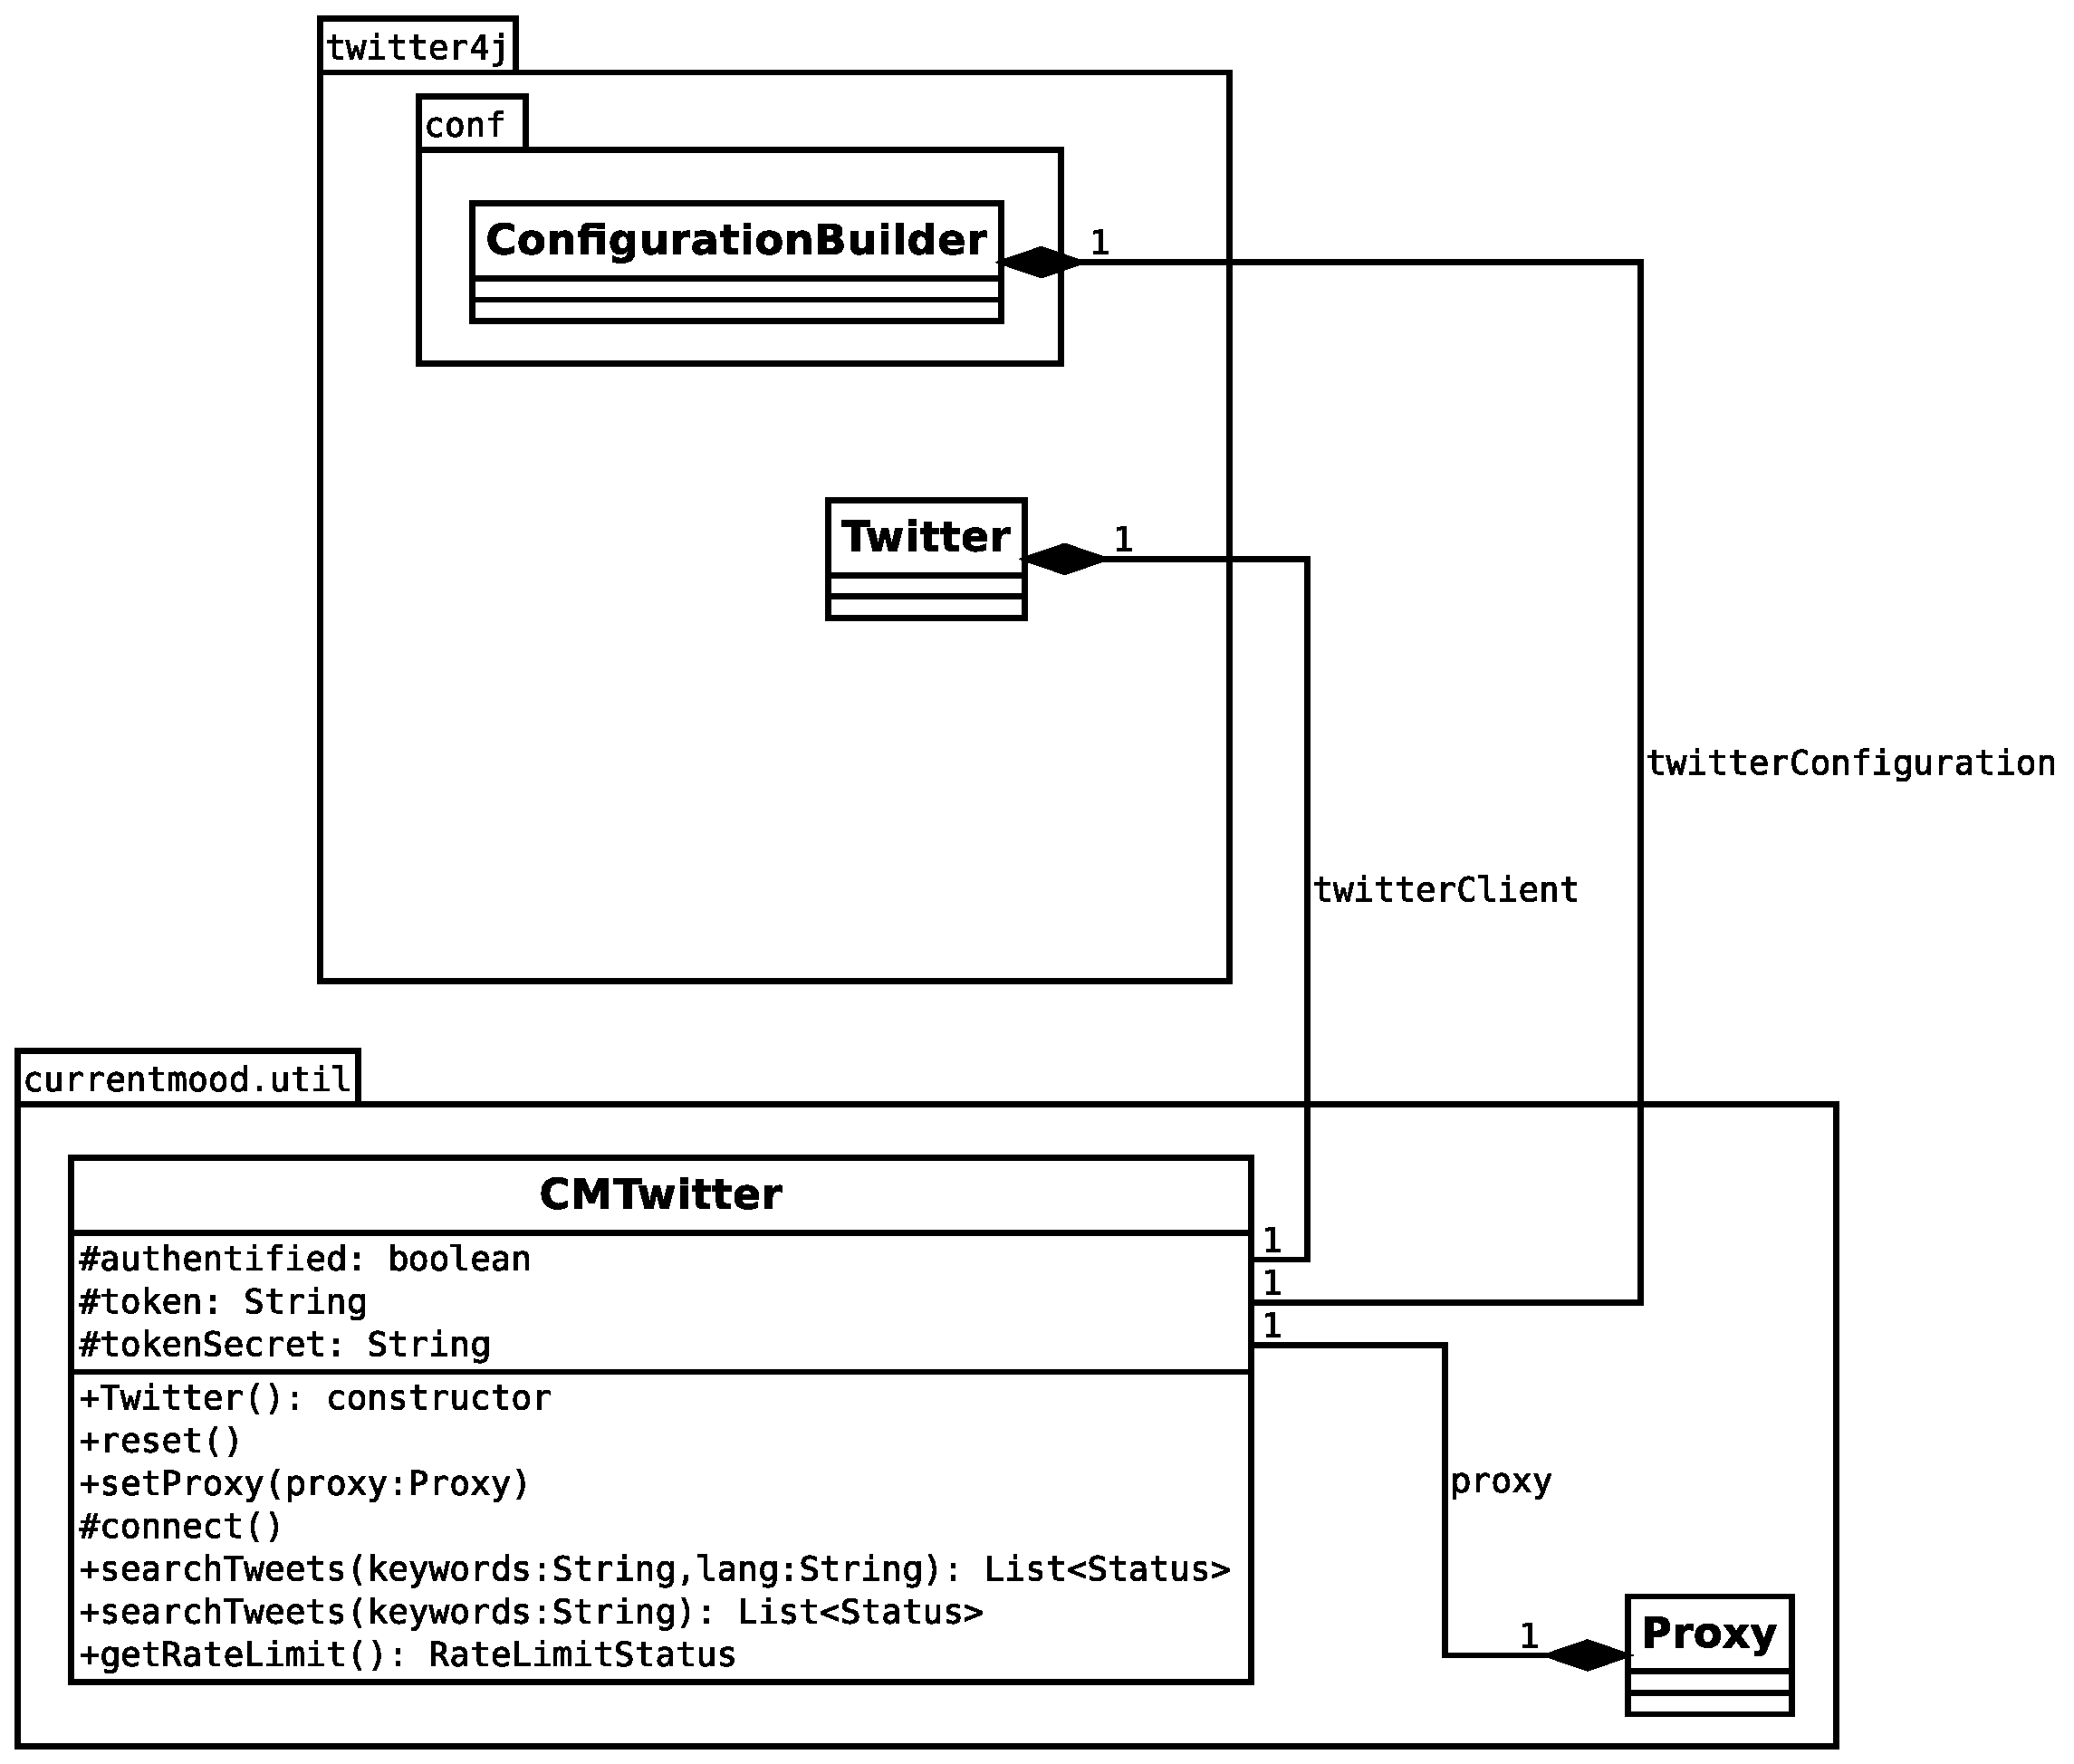
\includegraphics[width=\textwidth]{img/uml_cmtwitter.eps}
	\caption{Diagramme de classe montrant comment nous interfaçons Twitter4J}
	\label{uml_cmtwitter}
\end{figure}

Cela nous permet d'utiliser l'API de Twitter à l'aide de trois méthodes
principales seulement au lieu d'une dizaine:

\begin{itemize}
	\item
		\texttt{setProxy()} afin de donner les paramètres proxy à Twitter4J;
	\item
		\texttt{connect()} afin d'établir la connexion avec l'API de Twitter;
	\item
		\texttt{searchTweets()} afin d'utiliser la fonction de recherche de
		l'API de Twitter.
\end{itemize}

La méthode \texttt{reset()}, quant à elle, est utilisée par les méthodes
précédentes afin de permettre d'effectuer plusieurs requêtes. En effet, nous
avons pu remarquer que l'objet \texttt{ConfigurationBuilder} périme après chaque
requête, nous obligeant à le recréer avant d'effectuer une nouvelle requête.

L'utilisation de cette classe s'effectue en trois étapes principales.

Tout d'abord, on configure si nécessaire les paramètres proxy à l'aide de la
méthode \texttt{setProxy()}. Cette dernière donne lesdits paramètres à l'objet
\texttt{ConfigurationBuilder}.

Ensuite, on appelle la méthode \texttt{connect()} qui utilise l'objet
\texttt{ConfigurationBuilder} pour obtenir une instance de \texttt{Twitter}.

C'est cette instance qui est ensuite utilisée par \texttt{searchTweets()} qui
instancie un objet de Twitter4J permettant d'obtenir des tweets correspondant
à la recherche. Cette méthode retourne une liste d'objets \texttt{Status}
provenant de la librairie Twitter4J.

\newpage
\section{La classe \texttt{Tweet}}

Nous nous sommes rapidement rendus compte que Twitter4J ne proposait aucune
classe implémentant l'interface \texttt{Status} que nous devons manipuler. De
plus, les objets que nous en obtenons contient de nombreuses informations qui ne
nous sont pas utiles, tandis que d'autres nous étaient nécessaires mais
n'y étaient pas présents.

Nous avons donc créé une classe indépendante de Twitter4J, \texttt{Tweet}, qui
réponde à ce besoin (figure~\ref{uml_tweet}). Elle est utilisée dans toute l'application afin de contenir
chaque tweet.

\begin{figure}
	\centering
	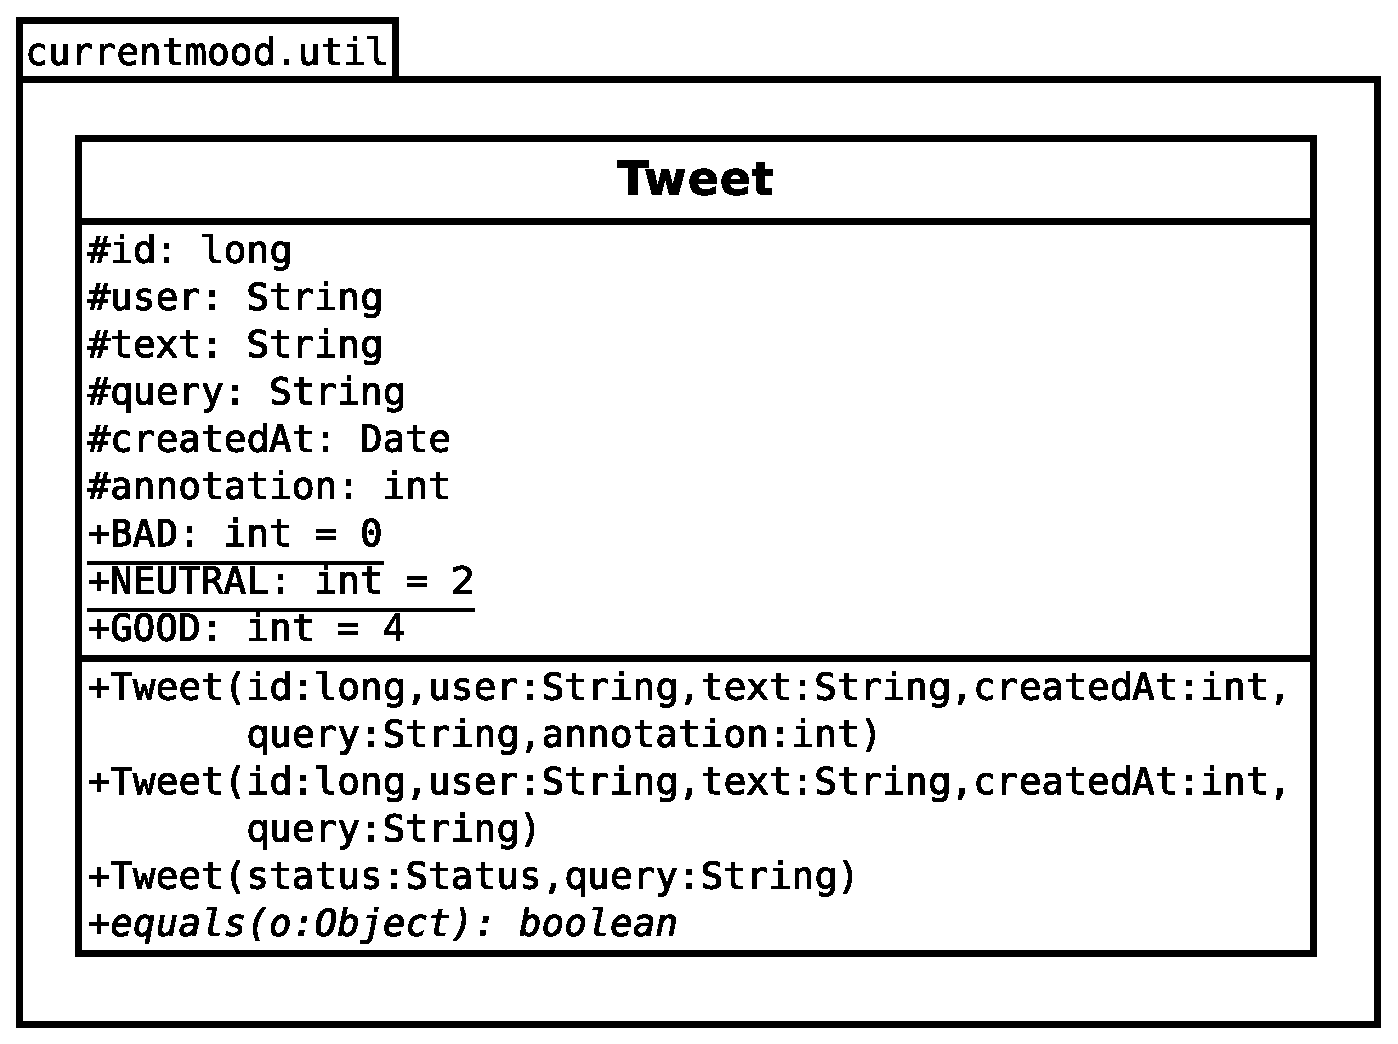
\includegraphics[width=9cm]{img/uml_tweet.eps}
	\caption{La classe \texttt{Tweet}}
	\label{uml_tweet}
\end{figure}

Cette classe est surtout composée d'accesseurs permettant d'accéder à chaque
propriété du tweet. Ses deux premiers constructeurs permettent de créer un objet
à partir de données déjà connues (typiquement lors de l'ouverture d'un fichier
CSV), tandis que le troisième permet d'obtenir un objet \texttt{Tweet} à partir
d'un objet \texttt{Status} généré par Twitter4J.

Nous avons également surchargé la méthode \texttt{equals()} de la super-classe
\texttt{Object} afin de permettre la comparaison de l'objet courant avec un
autre objet \texttt{Tweet}. Cela nous sera nécessaire pour certaines actions par
la suite.

% -----------------------------------------------------------------------------
\chapter{La base d'apprentissage}

\section{Le nettoyage des tweets}

L'annotation automatique se basant sur une base d'apprentissage construite
manuellement, il est primordial d'avoir une base de données saine pour éviter
les erreurs d'interprétation. Cela passe par un nettoyage des tweets afin de
limiter le «~bruit~».

Lors de la sauvegarde des tweets annotés manuellement dans un fichier CSV, nous
passons par une étape consistant à supprimer tout ce qui peut gêner
l'interprétation du tweet ou la lecture du fichier CSV.

Ainsi, nous supprimons:

\begin{itemize}
	\item
		Les retours à la ligne (pour respecter le format CSV)
	\item
		Les smileys \texttt{:)}, \texttt{:(}, \texttt{:D}, \texttt{:')},
		\texttt{:'(} et \texttt{:'D}
	\item
		Les liens hypertextes
	\item
		Les \texttt{@usernames}
	\item
		Les hashtags
	\item
		La ponctuation
	\item
		Les symboles monnétaires principaux (\euro, \$, £)
	\item
		Les pourcentages
\end{itemize}

Une fois ce nettoyage effectué, nous pouvons alors utiliser cette base de tweets
pour annoter automatiquement d'autres tweets selon quatre méthodes qui seront
traitées dans la
partie~\ref{chapter-classifications}~(page~\pageref{chapter-classifications}).
Ce nettoyage permet également d'enregistrer les tweets dans un fichier CSV sans
casser son format (en supprimant notamment les retours à la ligne et les
virgules).

\section{Le fichier CSV}

Pour gérer la base de données, il a été décidé de sauvegarder les messages
annotés dans un fichier CSV\footnote{\textit{Comma-separated values}}. Ce type
de fichier a pour principal avantage d'être relativement léger et facile à lire
par programmation.

Les données à sauvegarder étant globalement celles contenues dans les objets
\texttt{Tweet}, l'ordre de sauvegarde sera donc le suivant:

\begin{enumerate}
	\item
		Le numéro d'identification du tweet
	\item
		Le nom de l'auteur du tweet
	\item
		Le contenu du tweet
	\item
		La date et l'heure du tweet, sous la forme d'un
		\textit{timestamp}\footnote{Nombre de secondes depuis le 
		1\ier{} janvier 1970, 0 h 00 min 00 s GMT}. S'il est nul, il est
		ignoré.
	\item
		La recherche qui a permis de trouver le tweet
	\item
		L'annotation du tweet
\end{enumerate}

L'annotation du tweet est enregistré sous la forme d'un nombre dont la valeur
est précisé par le tableau~\ref{tableau-valeurs-annotation}.

\begin{table}[h]
	\centering
	\begin{tabular}{c c}
		\textbf{Valeur de l'annotation}	& \textbf{Humeur du tweet}\\
		\midrule
		$0$				& Mauvais\\
		\midrule
		$2$				& Neutre\\
		\midrule
		$4$				& Bon
	\end{tabular}
	\caption{Valeur de l'annotation selon l'humeur du tweet}
	\label{tableau-valeurs-annotation}
\end{table}

\section{Classifier manuellement un tweet dans \CMName}
Après avoir chargé des tweets provenant de Twitter dans \CMName, il suffit de
cliquer droit sur un tweet et, dans le menu contextuel, de choisir
\textit{Annoter à la main} et l'annotation que l'on souhaite ajouter au tweet
(figure~\ref{capture-annoter-a-la-main}).

\begin{figure}
	\centering
	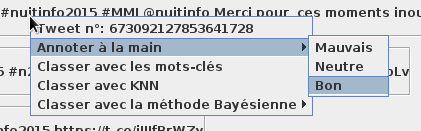
\includegraphics{img/capture-annoter-a-la-main.png}
	\caption{Menu contextuel permettant d'annoter un tweet à la main}
	\label{capture-annoter-a-la-main}
\end{figure}

% -----------------------------------------------------------------------------
\chapter{Classification automatique des tweets}
\label{chapter-classifications}

\section{Classification par mots-clés}
La classification par mots-clés est la plus simple des méthodes de
classification. Elle consiste à se baser sur une liste de mots définis dans un
fichier pour déterminer l'humeur d'un tweet.

Sa stratégie est des plus simples: pour un tweet donné, on recherche
chacun de ses mots dans un dictionnaire définissant des mots positifs et des
mots négatifs. Leur nombre respectifs déterminera alors l'humeur du tweet. Par
exemple, un tweet contenant 3 mots considérés positifs et 5 mots considérés
négatifs sera annoté négatif. Un tweet qui contiendrait un même nombre de mots
positifs et négatifs est considéré comme étant neutre.

Cette méthode a pour principaux avantages d'être très simples à mettre en œuvre
et de ne pas nécessiter de base d'apprentissage de tweets. Seul un dictionnaire
de mots positifs et de mots négatifs est nécessaire pour pouvoir annoter un
tweet.

Son inconvénient majeur est que le dictionnaire doit être particulièrement
fourni en mots positifs et négatifs pour être efficace. De plus, réduire une
phrase complète à de simples mots-clés ne permet pas de prendre en compte le
sens général de la carte. Prenons par exemple le tweet suivant :

\begin{quote}
	Génial, ma banque m'a refusé mon crédit…
\end{quote}

On remarque bien que ce tweet est plutôt négatif. Cependant, la présence du mot
\textit{génial} peut influencer la classification finale, ce qui peut déboucher,
ici, à un faux positif.

\section{Classification par la méthode KNN}
La méthode des $k$ plus proches voisins, ou KNN\footnote{$k$-nearest neighbor},
est une méthode consistant à exploiter la base d'apprentissage en comptant le
nombre de mots en commun entre un tweet à annoter et chaque tweet de la base.

L'humeur du tweet est alors déterminée selon l'humeur des $k$ tweets
avec lesquels il a le plus de mots en commun.

Pour ce faire, l'algorithme calcule la distance entre le tweet à annoter (que
l'on nommera $A$ par la suite) et chaque tweet de la base de données
en conservant les $k$ tweets les plus proches ($k$ étant un nombre
choisi par l'utilisateur). Il en déduit alors l'humeur du tweet $A$ en comparant
simplement le nombre de tweets positifs, neutres et négatifs parmi les $k$ plus
proches.

L'intérêt d'utiliser un nombre $k$ est que l'on utilise alors un nombre réduit
de tweets parmi ceux les plus proches, ce qui permet d'influer sur la précision
de l'algorithme.

Cette méthode a pour principal avantage d'être simple à mettre en œuvre.
Cependant, il peut être délicat de choisir une valeur pour $k$, qui peut
grandement influer sur le résultat. De plus, comme pour la méthode de
classification par mots-clés, le sens de la phrase n'est pas pris en compte.
Pis, il peut aussi être perturbé par certains mots n'apportant pas de sens
supplémentaire au message phrase et propres à la langue (articles, conjonctions
de coordination, prépositions...).

\section{Classification par la méthode bayésienne}


% -----------------------------------------------------------------------------

\end{document}
